\chapter{Structure, Guidelines, New Folder Setup}

\section{Directory Structure}

We briefly describe the directory structure of \Dumux in terms 
of subdirectories, source files, and tests. For more details, 
the Doxygen documentation should be considered. 
\Dumux comes in form of a DUNE module \texttt{dumux}. 
It has a similar structure as other DUNE modules like \texttt{dune-grid}. 
The following subdirectories are within the module's root directory, 
from now on assumed to be \texttt{/}: 
\begin{itemize}
\item \texttt{bin}: contains binaries, e.g. used for the automatic testing
\item \texttt{CMake}: the configuration options 
for building \Dumux using CMake. See the file \texttt{INSTALL.cmake} in 
the root directory of \texttt{dumux} for details. Of course, 
it is also possible to use the DUNE buildsystem just like for the other 
DUNE modules.
\item \texttt{doc}: contains the Doxygen documentation in \texttt{doxygen}, 
this handbook in \texttt{handbook}, and the \Dumux logo in various formats in 
\texttt{logo}. The html documentation produced by Doxygen can be accessed as usual, 
namely, by opening \texttt{doc/doxygen/html/index.html} with a web browser. 
\item \texttt{dumux}: the \Dumux source files. See Section \ref{sec:dumux} for details. 
\item \texttt{test}: tests for each numerical model and the property system. 
See Section \ref{sec:test} for details. 
\item \texttt{tutorial}: contains the tutorials described in Chapter \ref{chp:tutorial}. 
\end{itemize}



\subsection{The directory \texttt{dumux}}\label{sec:dumux}

The directory \texttt{dumux} contains the \Dumux source files. It consists of the following subdirectories (see Figure \ref{fig:dumux-structure}): 

\begin{itemize} 

\item \texttt{implicit}:
the general fully implicit method is contained in the subdirectory \texttt{common}. 
The subdirectories \texttt{box} and \texttt{cellcentered} contain the code for the according 
discretization types. They also contain files \texttt{..fvelementgeometry.hh} employed 
by the box or cc method to extract the dual mesh geometry information out of the primal one. 
Each of the other subdirectories contain a derived specific numerical model. 
% The files \texttt{pdelabboxassembler.hh} and \texttt{pdelabboxlocaloperator.hh} allow the use of the DUNE module \texttt{dune-pdelab}. 

\item \texttt{common}:
general stuff like the property system and the time management for the 
fully coupled as well as the decoupled models, 
% the interface for the Pardiso direct solver library \cite{Pardiso}, 
and the \texttt{start.hh} file that includes the common routine for starting a model called in the main function. 

\item \texttt{decoupled}:
 numerical models to solve the pressure equation as part of the fractional flow formulation. The specific models are contained 
 in corresponding subdirectories. In each model folder are subdirectories for the implicit pressure equation sorted by the employed discretization method, and for the explicit transport equation. The general decoupled formulation for the implicit pressure explicit transport formulation can be found in the subdirectory \texttt{common}.

% \item \texttt{fractionalflow}:
% the (non-compositional) fractional flow model, which utilizes the IMPES method 
% contained in the subdirectory \texttt{impes}.

% \item \texttt{functions}:
% the Crouzeix--Raviart function implemented in the style of \texttt{dune-disc}'s P1 function. 

% \item \texttt{fvgeometry}:
% employed by the box method to extract the dual mesh geometry information out of the 
% primal one. 

\item \texttt{io}: additional in-/output possibilities like restart files, gnuplot-interface 
and a VTKWriter extension. 

\item \texttt{material}: everything related to material parameters and 
constitutive equations. The properties of a pure chemical substance (e.g. water) or pseudo substance (e.g. air) can be found in the subdirectory \texttt{components} with the base class \texttt{components/component.hh}. The fluidsytem in the folder \texttt{fluidsystems} collects the information from the respective component and binary coefficients files, and contains the fluid characteristics of phases (e.g. viscosity, density, enthalpy, diffusion coefficients) for compositional or non-compositional multi-phase flow. 

The base class for all spatially dependend variables -- like permeability and porosity  -- 
can be found in \texttt{spatialparams}. The base class in \texttt{implicitspatialparameters.hh} 
also provides spatial averaging routines. All other spatial properties are specified in the specific
 files of the respective models. Furthermore, the constitutive relations -- e.g. $p_c(S_w) $ -- are in \texttt{fluidmatrixinteractions}, 
while the necessary binary coefficients like the Henry coefficient or binary diffusion coefficients are definded in
 \texttt{binarycoefficients}.


\item \texttt{nonlinear}: Newton's method.


% \item \texttt{operators}: based on \texttt{dune-disc}, assembly operators for Crouzeix--Raviart 
% elements and mimetic finite differences. 
% 
% 
% \item \texttt{pardiso}: interface to the Pardiso direct solver library, \cite{Pardiso}. 
% 
% 
% \item \texttt{shapefunctions}:  Crouzeix--Raviart element shape functions. 
% 
% 
% \item \texttt{timedisc}: time discretization for the decoupled models. 
% 
% 
% \item \texttt{transport}: numerical models to solve the pressure equation 
% as part of the fractional flow formulation analogous to the \texttt{diffusion} 
% directory. Moreover, the compositional decoupled models are included here. 


\end{itemize}



\subsection{The directory \texttt{test}}\label{sec:test}


The directory \texttt{test} contains a test for each numerical model and for 
the property system. The tests for the property system can be found in \texttt{common}. 
The subfolder \texttt{implicit} contains tests for the fully 
coupled models (\texttt{1p},  \texttt{1p2c},  \texttt{2p},  \texttt{2p2c},  
\texttt{2p2cni},  \texttt{2pni}, \texttt{3p3c},  \texttt{3p3cni},  \texttt{mpnc} and \texttt{richards}), while the subdirectory \texttt{decoupled} corresponds to the decoupled models. 
Each subdirectory contains one or more program files \texttt{test\_*.cc}, where \texttt{*} usually is the 
name of the folder. Moreover, the problem definitions can be found 
in the \texttt{*problem.hh} files and the definition of the spatially dependent parameters in \texttt{*spatialparameters.hh}. Simply executing the tests should either run the 
full test or give a list of required command line arguments. After test execution, 
VTK output files should have been generated. 
For more detailed descriptions of the tests, the problem definitions and their corresponding 
Doxygen documentation should be considered. 

\begin{sidewaysfigure}
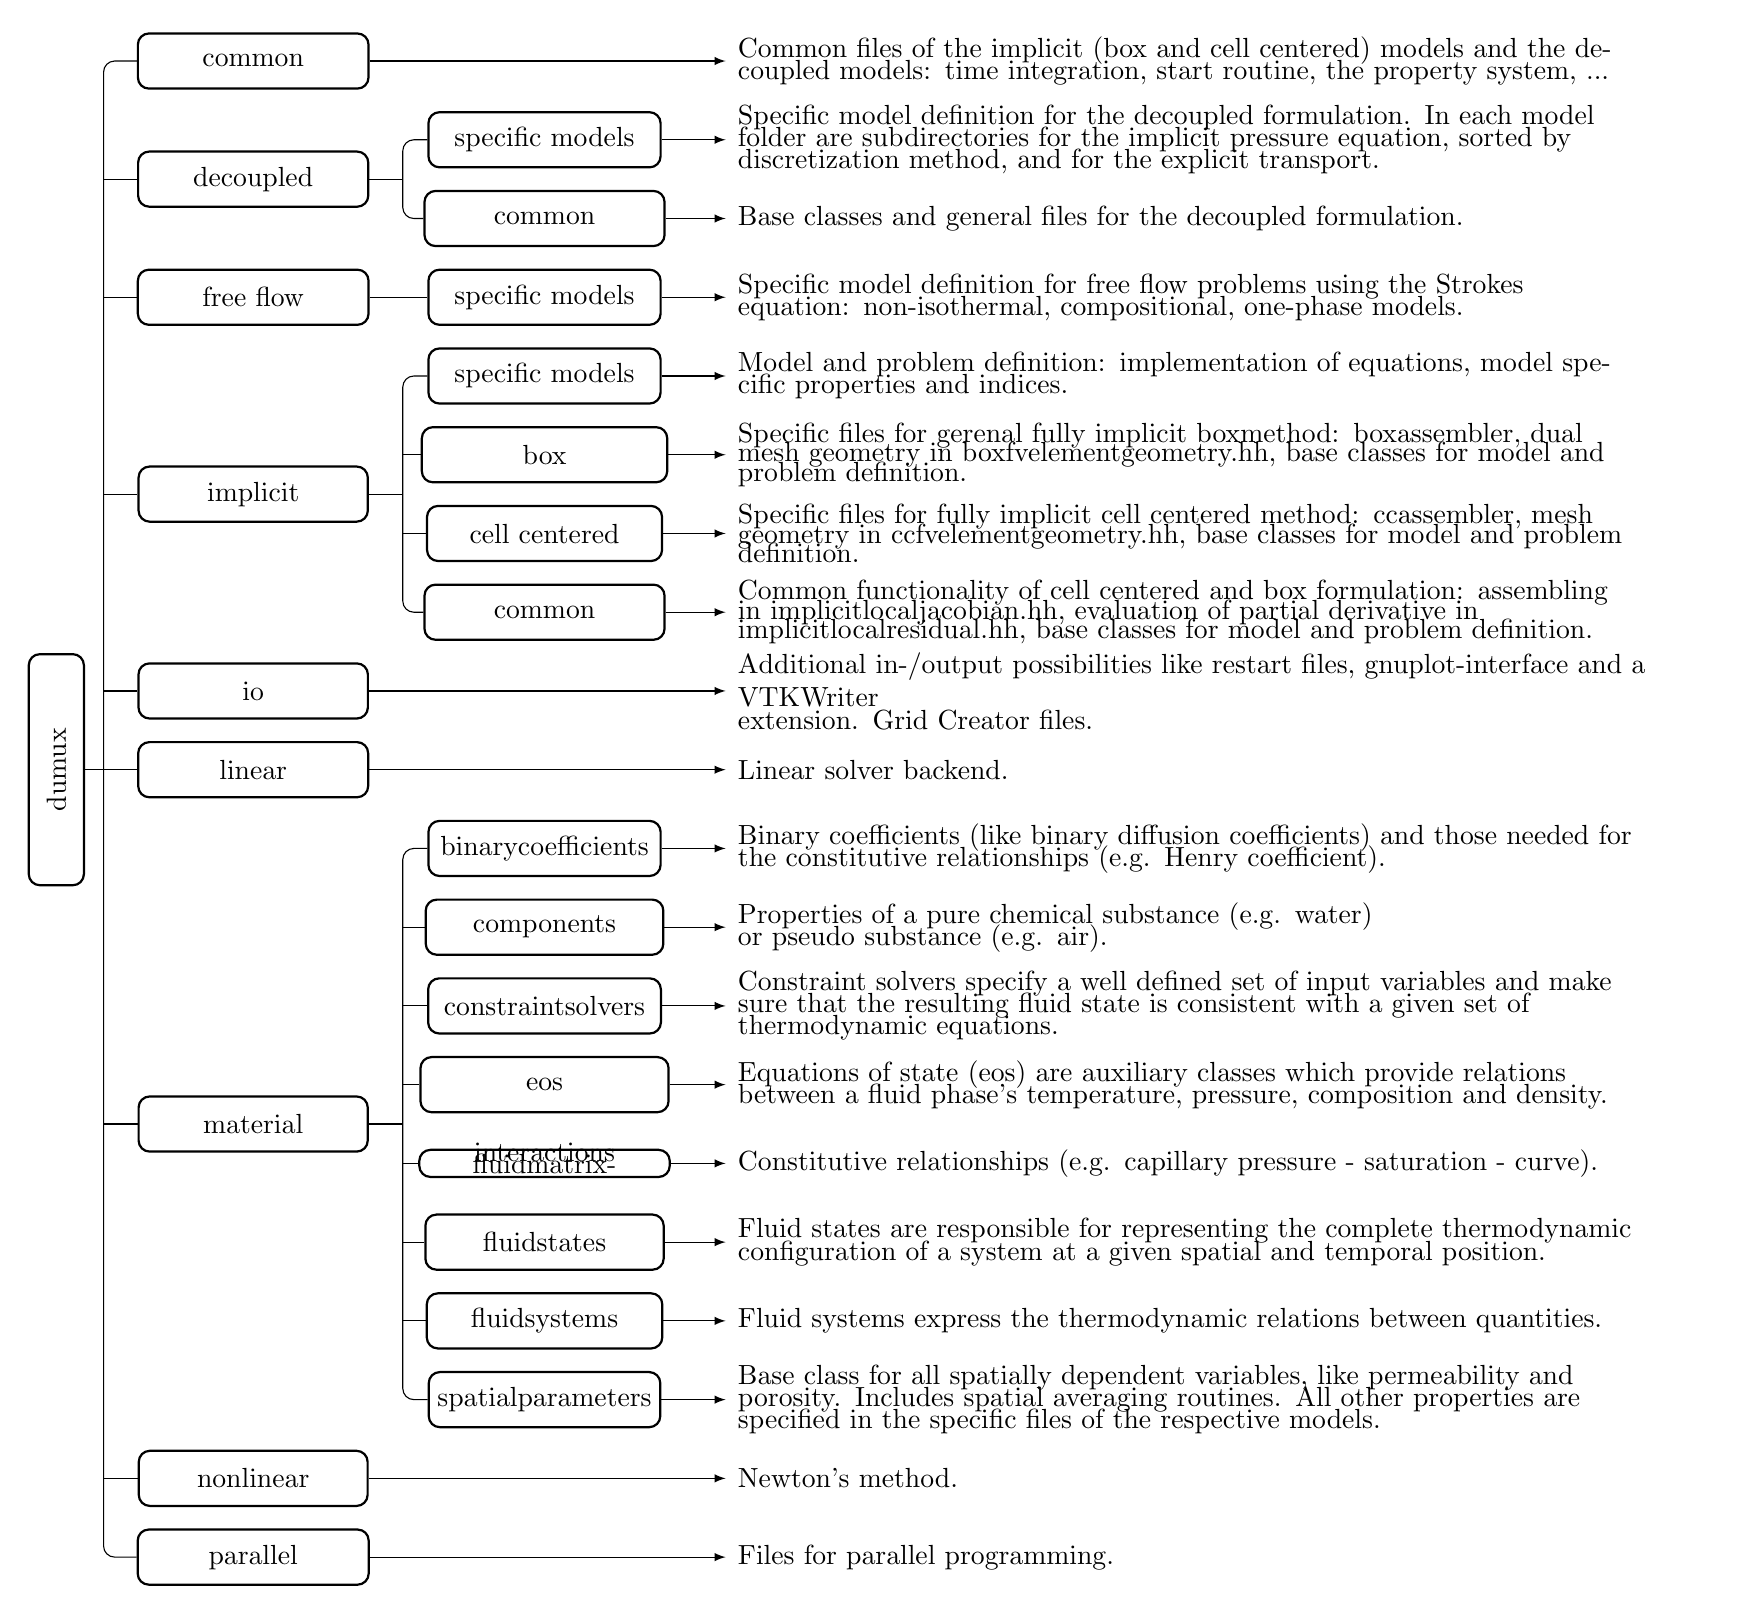
\begin{tikzpicture}[>=latex,inner xsep=0.15cm,rounded corners]
\node [minimum height=0.7cm,draw,inner xsep=0.94cm,rotate=90,thick] (d) at(-2,0) {dumux};
\node [minimum height=0.7cm,draw,inner xsep=1.03cm,thick] (lin) at(0.5,0) {linear};
\node [minimum height=0.7cm,draw,inner xsep=1.32cm,thick] (io) at(0.5,1) {io};

\node [minimum height=0.7cm,draw,inner xsep=0.87cm,thick] (imp) at(0.5,3.5) {implicit};
 \node [minimum height=0.7cm,draw,inner xsep=0.88cm,thick] (c1) at(4.2,2) {common};
 \node [minimum height=0.7cm,draw,inner xsep=0.54cm,thick] (cell) at(4.2,3) {cell centered};
 \node [minimum height=0.7cm,draw,inner xsep=1.28cm,thick] (box) at(4.2,4) {box};
 \node [minimum height=0.7cm,draw,inner xsep=0.33cm,thick] (spec1) at(4.2,5) {specific models};

\node [minimum height=0.7cm,draw,inner xsep=0.82cm,thick] (free) at(0.5,6) {free flow};
  \node [minimum height=0.7cm,draw,inner xsep=0.33cm,thick] (spec2) at(4.2,6) {specific models};

\node [minimum height=0.7cm,draw,inner xsep=0.7cm,thick] (dec) at(0.5,7.5) {decoupled};
 \node [minimum height=0.7cm,draw,inner xsep=0.88cm,thick] (c2) at(4.2,7) {common};
 \node [minimum height=0.7cm,draw,inner xsep=0.33cm,thick] (spec3) at(4.2,8) {specific models};

\node [minimum height=0.7cm,draw,inner xsep=0.82cm,thick] (c3) at(0.5,9) {common};

\node [minimum height=0.7cm,draw,inner xsep=0.82cm,thick] (m) at(0.5,-4.5) {material};
 \node [minimum height=0.7cm,draw,thick] (bin) at(4.2,-1) {binarycoefficients};
 \node [minimum height=0.7cm,draw,inner xsep=0.6cm,thick] (comp) at(4.2,-2) {components};
 \node [minimum height=0.7cm,draw,inner xsep=0.2cm,thick] (con) at(4.2,-3) {constraintsolvers};
 \node [minimum height=0.7cm,draw,inner xsep=1.34cm,thick] (eos) at(4.2,-4) {eos};
 \node [inner ysep=0.05cm,draw,text width=2cm,align=center,inner xsep=0.59cm,thick] (fi) at(4.2,-5) {fluidmatrix-\\[-16pt]interactions};
 \node [minimum height=0.7cm,draw,inner xsep=0.73cm,thick] (fstate) at(4.2,-6) {fluidstates};
 \node [minimum height=0.7cm,draw,inner xsep=0.56cm,thick] (fsys) at(4.2,-7) {fluidsystems}; 
 \node [minimum height=0.7cm,draw,inner xsep=0.11cm,thick] (s) at(4.2,-8) {spatialparameters}; 

\node [minimum height=0.7cm,draw,inner xsep=0.74cm,thick] (non) at(0.5,-9) {nonlinear}; 
\node [minimum height=0.7cm,draw,inner xsep=0.9cm,thick] (para) at(0.5,-10) {parallel};

\draw (d)--(lin);
\draw (-1.4,0)--(-1.4,9)--(c3);
\draw (-1.4,0)--(-1.4,-10)--(para);
\draw (-1.4,7.5)--(dec);
\draw (-1.4,6)--(free);
\draw (-1.4,3.5)--(imp);
\draw (-1.4,1)--(io);
\draw (-1.4,-4.5)--(m);
\draw (-1.4,-9)--(non);

\draw (dec)--(2.4,7.5);
\draw (spec3)--(2.4,8)--(2.4,7)--(c2);
\draw (free)--(spec2);
\draw (imp)--(2.4,3.5);
\draw (spec1)--(2.4,5)--(2.4,2)--(c1);
\draw (box)--(2.4,4);
\draw (cell)--(2.4,3);
\draw (m)--(2.4,-4.5);
\draw (bin)--(2.4,-1)--(2.4,-8)--(s);
\draw (comp)--(2.4,-2);
\draw (con)--(2.4,-3);
\draw (eos)--(2.4,-4);
\draw (fi)--(2.4,-5);
\draw (fstate)--(2.4,-6);
\draw (fsys)--(2.4,-7);

\draw [->](c3)--(6.5,9) node [right,text width=12.5cm,align=left] 
  {Common files of the implicit (box and cell centered) models and the de-\\[-4pt]coupled models: time integration, start routine, the  property system, ...};
\draw [->](spec3)--(6.5,8) node [right,text width=12.5cm,align=left] 
  {Specific model definition for the decoupled formulation. In each model \\[-4pt]folder are subdirectories for the implicit pressure  equation, sorted by \\[-4pt]discretization method, and for the explicit transport.};
\draw [->](c2)--(6.5,7) node [right,text width=12.5cm,align=left] 
  {Base classes and general files for the decoupled formulation.};
\draw [->](spec2)--(6.5,6) node [right,text width=12.5cm,align=left] 
  {Specific model definition for free flow problems using the Strokes \\[-4pt]equation: non-isothermal, compositional, one-phase models.};
\draw [->](spec1)--(6.5,5) node [right,text width=12.5cm,align=left] 
  {Model and problem definition: implementation of equations, model spe-\\[-4pt]cific properties and indices.};
\draw [->](box)--(6.5,4) node [right,text width=12.5cm,align=left] 
  {Specific files for gerenal fully implicit boxmethod: boxassembler, dual \\[-5pt]mesh geometry in boxfvelementgeometry.hh, base classes for model and \\[-5pt]problem definition.};
\draw [->](cell)--(6.5,3) node [right,text width=12.5cm,align=left] 
  {Specific files for fully implicit cell centered method: ccassembler, mesh \\[-5pt]geometry in ccfvelementgeometry.hh, base classes for model and problem \\[-5pt]definition.};
\draw [->](c1)--(6.5,2) node [right,text width=12.5cm,align=left] 
  {Common functionality of cell centered and box formulation: assembling \\[-5pt]in implicitlocaljacobian.hh, evaluation of partial derivative in \\[-5pt]implicitlocalresidual.hh, base classes for model and problem definition.};
\draw [->](io)--(6.5,1) node [right,text width=12.5cm,align=left] 
  {Additional in-/output possibilities like restart files, gnuplot-interface and a VTKWriter \\[-4pt]extension. Grid Creator files.};
\draw [->](lin)--(6.5,0) node [right,text width=12.5cm,align=left] {Linear solver backend.};
\draw [->](bin)--(6.5,-1) node [right,text width=12.5cm,align=left] 
  {Binary coefficients (like binary diffusion coefficients) and those needed for \\[-4pt]the constitutive relationships (e.g. Henry coefficient).};
\draw [->](comp)--(6.5,-2) node [right,text width=12.5cm,align=left] 
  {Properties of a pure chemical substance (e.g. water) \\[-4pt]or pseudo substance (e.g. air).};
\draw [->](con)--(6.5,-3) node [right,text width=12.5cm,align=left] 
  {Constraint solvers specify a well defined set of input variables and make \\[-4pt]sure that the resulting fluid state is consistent with a given set of \\[-4pt]thermodynamic equations.};
\draw [->](eos)--(6.5,-4) node [right,text width=12.5cm,align=left] 
  {Equations of state (eos) are auxiliary classes which provide relations \\[-4pt]between a fluid phase's temperature, pressure, composition and density.};
\draw [->](fi)--(6.5,-5) node [right,text width=12.5cm,align=left] 
  {Constitutive relationships (e.g. capillary pressure - saturation - curve).};
\draw [->](fstate)--(6.5,-6) node [right,text width=12.5cm,align=left] 
  {Fluid states are responsible for representing the complete thermodynamic \\[-4pt]configuration of a system at a given spatial and temporal position.};
\draw [->](fsys)--(6.5,-7) node [right,text width=12.5cm,align=left] 
  {Fluid systems express the thermodynamic relations between quantities.};
\draw [->](s)--(6.5,-8) node [right,text width=12.5cm,align=left] 
  {Base class for all spatially dependent variables, like permeability and \\[-4pt]porosity. Includes spatial averaging routines. All other properties are \\[-4pt]specified in the specific files of the respective models.};
\draw [->](non)--(6.5,-9) node [right,text width=12.5cm,align=left] 
  {Newton's method.};
\draw [->](para)--(6.5,-10) node [right,text width=12.5cm,align=left] 
  {Files for parallel programming.};
\end{tikzpicture}
\caption{Structure of the directory \texttt{dumux} containing the \Dumux source files.}
\label{fig:dumux-structure}
\end{sidewaysfigure}

% \begin{landscape}
% \begin{figure}[hbt]
%   \centering 
%   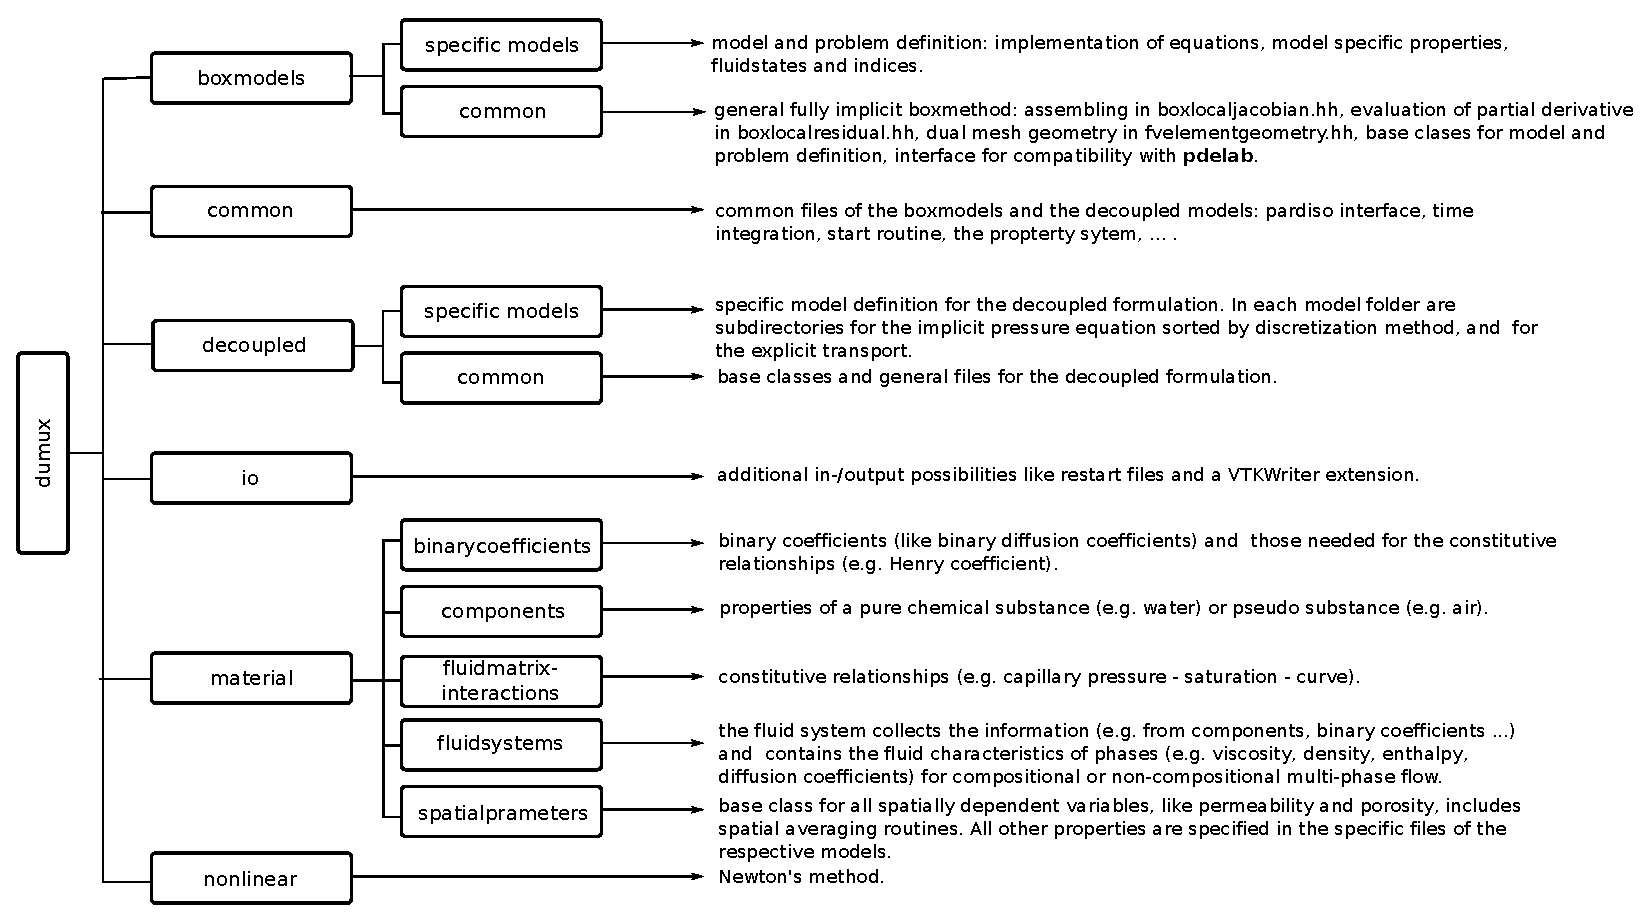
\includegraphics[width=\linewidth, keepaspectratio]{EPS/dumux_strucutre_flowchart_horizontal_explained.eps}
%   \caption{
%     \label{fig:dumux-structure}
%     Structure of the directory \texttt{dumux} containing the \Dumux source files.
%   }
% \end{figure}
% \end{landscape}

\section{Setup of a New Folder}

In this section setting up a new folder is described. In fact it is easy to create a new folder, but getting the build system to know the new folder takes some steps:

\begin{enumerate}[1)]
 \item create new folder with content
 \item adapt \verb+Makefile.am+
 \item insert new folder in \verb+Makefile.am+ of the directory above
 \item adapt \verb+configure.ac+ in the \verb+$DUMUX_ROOT+ (the directory you checked out, probably dumux)
 \item rerun dunecontrol / autogen for \Dumux
\end{enumerate}

\noindent In more detail:

\textbf{First} of all, the new folder including all relevant files needs to be created (see Section \ref{tutorial-coupled} and \ref{tutorial-decoupled} for description of a problem). 

\textbf{Second}, a new \verb+Makefile.am+ for the new Folder needs to be created. It is good practice to simply copy an existing file. For example the file \verb+$DUMUX_ROOT/test/2p/Makefile.am+ looks as follows:
\begin{verbatim}
bin_PROGRAMS = test_2p

test_2p_SOURCES = test_2p.cc
test_2p_CXXFLAGS = $(MPI_CPPFLAGS) 
test_2p_LDADD = $(MPI_LDFLAGS) 

include $(top_srcdir)/am/global-rules
\end{verbatim}

All occurrences of \verb+test_2p+ need to be replaced by the name of the new project, e.g. \verb+New_Project+. At least if the name of the source file as well as the name of the new project are \verb+New_Project+.

\textbf{Third}: In the directory above your new Project there is also a \verb+Makefile.am+ . In this file the subdirectories are listed. As you introduced a new subdirectory, it needs to be included here. In this case the name of the new Folder is \verb+New_Project+ . Don't forget the trailing backslash.

\begin{verbatim}
 SUBDIRS = . \
	  1p \
	  1p2c \
	  2p \
	  2p2c \
	  2p2cni \
	  2pni \
	New_Project \
...
\end{verbatim}

\textbf{Fourth}: In \verb+$DUMUX_ROOT+ there is a file \verb+configure.ac+. In this file, the respective Makefiles are listed. After a line reading

 \verb+AC_CONFIG_FILES([Makefile+ 

 \noindent a line, declaring a new Makefile, needs to be included. The Makefile itself will be generated automatically during the autogen run which is triggered by dunecontrol. For keeping track of the included files, inserting in alphabetical order is good practice. The new line could read: \verb+test/New_Project/Makefile+ 

\textbf{Fifth}: Recreate the build system by running dunecontrol as described in Section \ref{install}.

\paragraph{Committing a new folder to the Subversion repository}
For those who work with Subversion (svn) and want to commit a newly setup folder to the repository some basics are
given in this paragraph. For further reading please check out the Subversion User Manual found at \cite{APACHE-SUBVERSION-HP}
where you will also find a "High Speed Turorial" in the appendix. \\
The four most important commands are \texttt{svn checkout}, \texttt{svn update},  \texttt{svn add} 
and \texttt{svn commit}. The first one (\texttt{svn checkout}) you probably already know from the \Dumux installation.
It will create a copy of the trunk version from the svn server on your local system. Use \texttt{svn update} to get the
latest changes in the repository (commits from other users). In order to add a new folder to the repository the following
steps have to be taken:

\begin{enumerate}[1)]
 \item \texttt{svn update}: The first step is to update your \Dumux. You should execute this command in your
dumux-stable or dumux-devel folder.
 \item \texttt{svn add --depth=empty YOURFOLDER}: This command adds the folder without its content.
 \item In your folder: use \texttt{svn add YOURFILES} to add your files. Generally, you should only add
your header files (.hh), your source files (.cc), your input file (.input) and if required your grid file (.dgf).
\item Use \texttt{svn commit} from the directory level containing your folder. This uploads all your changes to the
svn server. You will be asked to briefly explain the content of your commit in an editor.
\end{enumerate}

The above shows you the necessary steps if you use the command line. There are also other tools providing a graphical 
user interface for using svn like kdesvn or eclipse. The necessary steps for adding and committing stay the same.
In the following some additional guidelines are shown which are not necessary but are good practice.
Especially if you plan on committing to the stable part of \Dumux you must follow these steps.

\begin{enumerate}[1)]
 \item use svn attributes to ignore files which are automatically created by a dunecontrol run
 \item test \texttt{make headercheck}
 \item test Doxygen
\end{enumerate}

\noindent In more detail:

\textbf{First}: The command \verb+svn status+ marks all files which are not under version control with a question mark. Because dunecontrol creates a lot of files automatically this output becomes crowded and one might overlook ``real'' files which have to be added (they also will not be shown by a \verb+svn status -q+).
For the stable part of \Dumux there is the rule to ignore and only to ignore the folder {\em .deps}, executables \texttt{test\_*}, and the files {\em Makefile} and {\em Makefile.in}.

How to set the svn attributes:
\begin{itemize}
 \item{\em eclipse}: right click on the file/folder $\rightarrow$ ``team'' $\rightarrow$ ``add to svn:ignore\dots''
 \item{\em kdesvn}: right click on the file/folder $\rightarrow$ ``ignore/unignore current item''
 \item{\em svn on shell}: \verb+svn propset svn:ignore FILETOIGNORE .+
\end{itemize}
Commit the changes for example in the command line with \verb+svn commit -m+ to the repository. It is also possible to use wildcards, e.\,g., if you want to ignore all vtu-files in your application folder in dumux-devel set \verb+FILETOIGNORE+ to \verb+'*.vtu'+. Remember that such an ignore is only allowed in dumux-devel and not in the stable dumux.

\textbf{Second}: It is good practice that every header includes everything it uses by itself and does not rely on the includes from headers that are included by themselves. This can be tested with \texttt{make headercheck} and should be done before committing to stable dumux. To test a specific header, use \texttt{make} \texttt{headercheck} \texttt{HEADER=} and add the header's path.

\textbf{Third}: Run \texttt{make doc} in the \texttt{\$DUMUX\_ROOT} directory to generate the class documentation by Doxygen. Have a look into \texttt{\$DUMUX\_ROOT/doc/doxygen/doxyerror.log} whether one of your files have errors or are causing warnings. Please fix them.

\section{Parameter Files in \Dumux}
\label{sec:inputFiles}
\Dumux simulations can be run with the use parameter files. Here basic information how to set,
extend, and improve your problem by using parameter files.
A list of all available parameters is provided in the \texttt{doxygen} documentation
of the file \texttt{parameterfile}, which is accessible via \texttt{Modules -> Parameters}.

\subsection{Advantages of Parameter Files}
Parameter files are worth of taking a closer look at, because using then considerably
improves the workflow.

\begin{itemize}
  \item The parameter file is read in by the compiled program. This way you can change
        values without having to recompile the whole application.
  \item With a very generic model, you can use different input files for defining different
        setups and always use the same program.
  \item You can use the parameter file in order to back up parameters that you used for
        a certain model run.
\end{itemize}

\subsection{Changing Parameters}
After having run the example application from section \ref{quick-start-guide} you will
get the following output at the end of the simulation run
\footnote{If you did not get the output, restart the application the following way:
\texttt{./test{\_}box2p -parameterFile ./test\_box2p.input -PrintParameters 1},
this will print the parameters once your simulation is finished}
:
\begin{lstlisting}[style=Bash]
# Run-time specified parameters:
[ Grid ]
File = "./grids/test_2p.dgf"
[ Implicit ]
EnableJacobianRecycling = "1"
EnablePartialReassemble = "1"
[ Problem ]
Name = "lensbox"
[ SpatialParams ]
LensLowerLeftX = "1.0"
LensLowerLeftY = "2.0"
LensUpperRightX = "4.0"
LensUpperRightY = "3.0"
[ TimeManager ]
DtInitial = "250"
TEnd = "3000"
# Compile-time specified parameters:
[ Implicit ]
EnableHints = "0"
MassUpwindWeight = "1"
MaxTimeStepDivisions = "10"
MobilityUpwindWeight = "1"
NumericDifferenceMethod = "1"
UseTwoPointFlux = "0"
[ LinearSolver ]
MaxIterations = "250"
PreconditionerRelaxation = "1"
ResidualReduction = "1e-06"
Verbosity = "0"
[ Newton ]
EnableResidualCriterion = "0"
EnableShiftCriterion = "1"
MaxRelativeShift = "1e-08"
MaxSteps = "18"
ResidualReduction = "1e-05"
SatisfyResidualAndShiftCriterion = "0"
TargetSteps = "10"
UseLineSearch = "0"
WriteConvergence = "0"
[ Problem ]
EnableGravity = "1"
[ TimeManager ]
MaxTimeStepSize = "1.79769e+308"
[ Vtk ]
AddVelocity = "0"
\end{lstlisting}

A number of things can be learned from this. Most prominently it tells you the parameters,
that can easily be added to the input file without having to change anything in the source code.
The output will tell you, which parameters are available to the problem and whether they have
been specified
\begin{itemize}
  \item \emph{run-time} via your input file
  \item \emph{compile-time} and have not been overwritten by the input file
  \item in your input file, but are \emph{UNUSED} by the simulation
\end{itemize}
For example by adding
\begin{lstlisting}[style=Bash]
[ Newton ]
MaxRelativeShift = "1e-11"
\end{lstlisting}
to the input file you can specify that the Newton solver considers itself converged for an
error a thousand times smaller.

The \emph{UNUSED} warning
\begin{lstlisting}[style=Bash]
# UNUSED parameters:
Problem.ImportantVariable = "42"
\end{lstlisting}
is important, because it shows that the application did not read in this value.
Maybe because it was attributed to the wrong group or there was a typo.
This feature is \emph{very} useful for debugging or spotting typos, like when you wanted
to overwrite one of the parameters listed under \texttt{Compile-time specified parameters}
and misspelled it in the input file, it will be listed in the \texttt{UNUSED parameters} section.

\subsection{Technical Issues on Parameters}
In case you want to learn more about how the input files work, please have a
look at the very helpful \Dune documentation, look for
\texttt{Dune::ParameterTree}.

The parameter tree can also be filled without the help of a text file.
Everything that is specified in a \Dumux input file can also be specified
directly on the command line. If there is also an input file, the respective
parameter on the command line has precedence.

All applications have a help message which you can read by giving
\texttt{--help}   as a command line argument to the application. A message
listing syntax and the mandatory input will be displayed on the command line.



\section{Restart \Dumux Simulations}
\label{sec:restartSimulations}
Using the restart capability of \Dumux can be advantageous for computationally
expensive or time consuming simulations, because you can restart the simulation
from a specific point in time and e.g. extend the simulation beyond the originally
end of simulation. What you need is a \texttt{*.drs} file (which contains the
all necessary restart information.
Then you can simply restart a simulation via
\begin{lstlisting}[style=Bash]
./test_program -ParameterFile test_program.input -TimeManager.Restart RESTART_TIME
\end{lstlisting}
To the test restart behavior e.g. use the \texttt{test\_box1p2cni} problem
in the \texttt{test/implicit/1p2c} folder.
You get the \texttt{RESTART\_TIME} from the name of your \texttt{.drs} file.
Please note, that restarting will only work by giving a exact time from
an existing restart file.
Depending on your type of model, you should get a \texttt{.drs} file every
5th or 10th time step. If this not frequently enough, you can change it
by using the following function into your problem header:
\begin{lstlisting}[style=DumuxCode]
/*!
 * \brief Returns true if a restart file should be written to
 *        disk.
 */
bool shouldWriteRestartFile() const
{
  return true;
}
\end{lstlisting}


\section{Guidelines} 

This section quotes the DUNE coding guidelines found at \cite{DUNE-HP}. 
These guidelines also should be followed by every \Dumux developer and user. 
"In order to keep the code maintainable we have decided upon a set of coding rules. 
Some of them may seem like splitting hairs to you, but they do make it much easier 
for everybody to work on code that hasn't been written by oneself.

\begin{itemize}
\item Naming: 
\begin{itemize}
\item Variables: Names for variables should only consist of letters and digits. The first letter should be a lower case one. If your variable names consists of several words, then the first letter of each new word should be capital. As we decided on the only exception are the begin and end methods.
\item Private Data Variables: Names of private data variables end with an underscore.
\item Typenames: For typenames, the same rules as for variables apply. The only difference is that the first letter should be a capital one.
\item Macros: The use of preprocessor macros is strongly discouraged. If you have to use them for whatever reason, please use capital letters only.
\item The Exlusive-Access Macro: Every header file traditionally begins with the definition of a preprocessor constant that is used to make sure that each header file is only included once. If your header file is called 'myheaderfile.hh', this constant should be DUNE\_MYHEADERFILE\_HH.
\item Files: Filenames should consist of lower case letters exclusively. Header files get the suffix .hh, implementation files the suffix .cc
\end{itemize}
\item Documentation:
      Dune, as any software project of similar complexity, will stand and fall with the quality of its documentation.
Therefore it is of paramount importance that you document well everything you do! We use the doxygen system to extract easily-readable documentation from the source code. Please use its syntax everywhere. In particular, please comment all
\begin{itemize}
\item Method Parameters
\item Template Parameters
\item Return Values
\item Exceptions thrown by a method
 \end{itemize}
     Since we all know that writing documentation is not well-liked and is frequently defered to some vague 
'next week', we herewith proclaim the Doc-Me Dogma . It goes like this: Whatever you do, and in whatever hurry you 
happen to be, please document everything at least with a {\verb /** $\backslash$todo Please doc me! */}. That way at least the absence 
of documentation is documented, and it is easier to get rid of it systematically.
\item Exceptions:
      The use of exceptions for error handling is encouraged. Until further notice, all exceptions thrown are DuneEx.
\item Debugging Code:
      Global debugging code is switched off by setting the symbol NDEBUG. In particular, all asserts are 
automatically removed. Use those asserts freely!" 
\end{itemize}

